% Options for packages loaded elsewhere
\PassOptionsToPackage{unicode}{hyperref}
\PassOptionsToPackage{hyphens}{url}
\PassOptionsToPackage{dvipsnames,svgnames,x11names}{xcolor}
\PassOptionsToPackage{space}{xeCJK}
\documentclass[
  10pt,
]{article}
\usepackage{xcolor}
\usepackage[margin=0.7in]{geometry}
\usepackage{amsmath,amssymb}
\setcounter{secnumdepth}{-\maxdimen} % remove section numbering
\usepackage{iftex}
\ifPDFTeX
  \usepackage[T1]{fontenc}
  \usepackage[utf8]{inputenc}
  \usepackage{textcomp} % provide euro and other symbols
\else % if luatex or xetex
  \usepackage{unicode-math} % this also loads fontspec
  \defaultfontfeatures{Scale=MatchLowercase}
  \defaultfontfeatures[\rmfamily]{Ligatures=TeX,Scale=1}
\fi
\usepackage{lmodern}
\ifPDFTeX\else
  % xetex/luatex font selection
  \setmainfont[]{Arial}
  \setmonofont[]{Consolas}
  \ifXeTeX
    \usepackage{xeCJK}
    \setCJKmainfont[]{Microsoft YaHei}
  \fi
  \ifLuaTeX
    \usepackage[]{luatexja-fontspec}
    \setmainjfont[]{Microsoft YaHei}
  \fi
\fi
% Use upquote if available, for straight quotes in verbatim environments
\IfFileExists{upquote.sty}{\usepackage{upquote}}{}
\IfFileExists{microtype.sty}{% use microtype if available
  \usepackage[]{microtype}
  \UseMicrotypeSet[protrusion]{basicmath} % disable protrusion for tt fonts
}{}
\makeatletter
\@ifundefined{KOMAClassName}{% if non-KOMA class
  \IfFileExists{parskip.sty}{%
    \usepackage{parskip}
  }{% else
    \setlength{\parindent}{0pt}
    \setlength{\parskip}{6pt plus 2pt minus 1pt}}
}{% if KOMA class
  \KOMAoptions{parskip=half}}
\makeatother
\usepackage{longtable,booktabs,array}
\usepackage{calc} % for calculating minipage widths
% Correct order of tables after \paragraph or \subparagraph
\usepackage{etoolbox}
\makeatletter
\patchcmd\longtable{\par}{\if@noskipsec\mbox{}\fi\par}{}{}
\makeatother
% Allow footnotes in longtable head/foot
\IfFileExists{footnotehyper.sty}{\usepackage{footnotehyper}}{\usepackage{footnote}}
\makesavenoteenv{longtable}
\usepackage{graphicx}
\makeatletter
\newsavebox\pandoc@box
\newcommand*\pandocbounded[1]{% scales image to fit in text height/width
  \sbox\pandoc@box{#1}%
  \Gscale@div\@tempa{\textheight}{\dimexpr\ht\pandoc@box+\dp\pandoc@box\relax}%
  \Gscale@div\@tempb{\linewidth}{\wd\pandoc@box}%
  \ifdim\@tempb\p@<\@tempa\p@\let\@tempa\@tempb\fi% select the smaller of both
  \ifdim\@tempa\p@<\p@\scalebox{\@tempa}{\usebox\pandoc@box}%
  \else\usebox{\pandoc@box}%
  \fi%
}
% Set default figure placement to htbp
\def\fps@figure{htbp}
\makeatother
\setlength{\emergencystretch}{3em} % prevent overfull lines
\providecommand{\tightlist}{%
  \setlength{\itemsep}{0pt}\setlength{\parskip}{0pt}}
\usepackage{bookmark}
\IfFileExists{xurl.sty}{\usepackage{xurl}}{} % add URL line breaks if available
\urlstyle{same}
\hypersetup{
  colorlinks=true,
  linkcolor={Maroon},
  filecolor={Maroon},
  citecolor={Blue},
  urlcolor={blue},
  pdfcreator={LaTeX via pandoc}}

\author{}
\date{}

\usepackage{float}
\usepackage{needspace}
\setCJKmonofont{Microsoft YaHei}
\Urlmuskip=0mu plus 2mu\relax
\renewcommand{\figurename}{图}
\begin{document}

\section{三种子训练完成：数据扩展、退化增强与质量复核结果}\label{ux4e09ux79cdux5b50ux8badux7ec3ux5b8cux6210ux6570ux636eux6269ux5c55ux9000ux5316ux589eux5f3aux4e0eux8d28ux91cfux590dux6838ux7ed3ux679c}

2026 年 11 月 15 日 · \href{completed-results.en.md}{English} ·
\href{completed-results.zh.pdf}{中文 PDF}

六个方案、三个共同随机种子的 18 组训练及开发集评价已全部完成。每组完成
2,400 次参数更新，后台队列于 10:29 UTC
结束。与训练初期的单种子观察相比，完整结果明确了三点：扩展数据稳定改善
LAG 和 KEH；恢复原来源采样比例对 AIROGS 有小幅收益，对 ODIR
的方向随训练阶段变化；退化增强提高合成失焦图上的表现，原图分类和人工复核的收益需要分别评价。

质量复核方面，18 个选中模型上，仅低质量分数识别错误的 AUROC 为
0.4923--0.5627，按疾病分数接近 0.5 排序为 0.8248--0.8976。在每次复核 411
张图的比较中，加入 FTHNet 质量分数比仅使用疾病分数的拟合方法多选中 −4 至
+4 个错误。这一轮的主要收益来自疾病模型与训练数据的改进。

\subsection{数据与实验设计}\label{ux6570ux636eux4e0eux5b9eux9a8cux8bbeux8ba1}

数据版本为 expanded\_20261113。原数据对照使用 10,338
张训练图，扩展方案使用 15,480 张。共同的模型验证集有 2,046
张图，用来选择权重；规则开发集有 2,053 张原图，包括 814 张阳性、1,239
张阴性和 1,917
个关联组，用来分析分类错误和复核方法。已确认的双眼、重拍或同图变体按关联组共同处理。疾病分数
p 越高表示模型越倾向判阳性；质量分数 q
越高表示模型预测照片质量越好。\href{../../../../proposal-1106.pdf}{项目提案}使用两种分数选择人工复核照片，本轮评价相同复核量下加入
q 的额外收益。最终测试安排在模型、分类阈值和复核规则固定之后。

五个主要来源的规则开发图为 AIROGS 773 张（380 阳性）、ODIR 305 张（28
阳性，19 个阳性关联组）、Kaggle 142 张（95 阳性）、LAG 481 张（169
阳性）、KEH 153 张（75 阳性）。其他来源合计 199
张，计入全体漏诊与误报。AIROGS
使用转诊标签，其他来源按各自疾病定义保留标签；来源内 AUROC
用来比较同一来源的阳性、阴性排序。

所有方案使用相同 ImageNet 初始化的 EfficientNet-B0、320 像素输入、最多
16 张一批、AdamW 学习率 0.0001。随机种子为
20261115、20261116、20261117，每 300
次更新保存权重和验证预测。一次更新是根据一批图像的误差调整参数；本次预算为
2,400 次更新。每组从保存的八次验证中，按 AIROGS、ODIR、Kaggle、LAG、KEH
的等权 AUROC 均值选择权重。

``65\% 原来源''表示采样时约 65\%
的图像出现次数来自原数据来源，其余来自新增池；两个池内均按来源、类别计数的平方根倒数采样。``混合''表示约一半图像随机接受照明、失焦或散射中的一种处理；``失焦''表示约一半图像接受失焦处理。无退化方案保留共同的翻转等基础训练变换。

下表用验证集选中的权重评价。验证均值和开发均值均指五来源等权
AUROC；漏诊和误报以 p \textgreater{} 0.5
判阳性，表中计数为三个种子的平均值。Brier 为预测分数与 0/1
疾病标签差值平方的均值，越低表示分数误差越小。

\Needspace{18\baselineskip}
\Needspace{8\baselineskip}
\begin{longtable}[]{@{}
  >{\raggedright\arraybackslash}p{(\linewidth - 12\tabcolsep) * \real{0.14285}}
  >{\raggedright\arraybackslash}p{(\linewidth - 12\tabcolsep) * \real{0.14285}}
  >{\raggedright\arraybackslash}p{(\linewidth - 12\tabcolsep) * \real{0.14285}}
  >{\raggedright\arraybackslash}p{(\linewidth - 12\tabcolsep) * \real{0.14285}}
  >{\raggedright\arraybackslash}p{(\linewidth - 12\tabcolsep) * \real{0.14285}}
  >{\raggedright\arraybackslash}p{(\linewidth - 12\tabcolsep) * \real{0.14285}}
  >{\raggedright\arraybackslash}p{(\linewidth - 12\tabcolsep) * \real{0.14285}}@{}}
\toprule\noalign{}
\begin{minipage}[b]{\linewidth}\raggedright
方案
\end{minipage} & \begin{minipage}[b]{\linewidth}\raggedright
选中更新数（三种子）
\end{minipage} & \begin{minipage}[b]{\linewidth}\raggedright
验证均值
\end{minipage} & \begin{minipage}[b]{\linewidth}\raggedright
开发均值
\end{minipage} & \begin{minipage}[b]{\linewidth}\raggedright
漏诊
\end{minipage} & \begin{minipage}[b]{\linewidth}\raggedright
误报
\end{minipage} & \begin{minipage}[b]{\linewidth}\raggedright
Brier
\end{minipage} \\
\midrule\noalign{}
\endhead
\bottomrule\noalign{}
\endlastfoot
原数据 & 1800 / 1800 / 1200 & 0.8886 & 0.8969 & 148.3 & 133.3 &
0.1039 \\
扩展数据 & 2400 / 1800 / 2100 & 0.9619 & 0.9646 & 69.0 & 97.3 &
0.0615 \\
65\% 原来源 & 2100 / 1800 / 2100 & 0.9608 & 0.9666 & 83.3 & 88.3 &
0.0613 \\
扩展＋混合 & 2400 / 1800 / 1500 & 0.9610 & 0.9619 & 85.3 & 91.3 &
0.0631 \\
65\%＋混合 & 2400 / 1200 / 2100 & 0.9634 & 0.9642 & 76.7 & 95.3 &
0.0608 \\
65\%＋失焦 & 2400 / 1500 / 2100 & 0.9623 & 0.9627 & 64.0 & 102.0 &
0.0617 \\
\end{longtable}

\subsection{扩展数据的收益与来源采样的取舍}\label{ux6269ux5c55ux6570ux636eux7684ux6536ux76caux4e0eux6765ux6e90ux91c7ux6837ux7684ux53d6ux820d}

\begin{figure}[H]
\centering
\pandocbounded{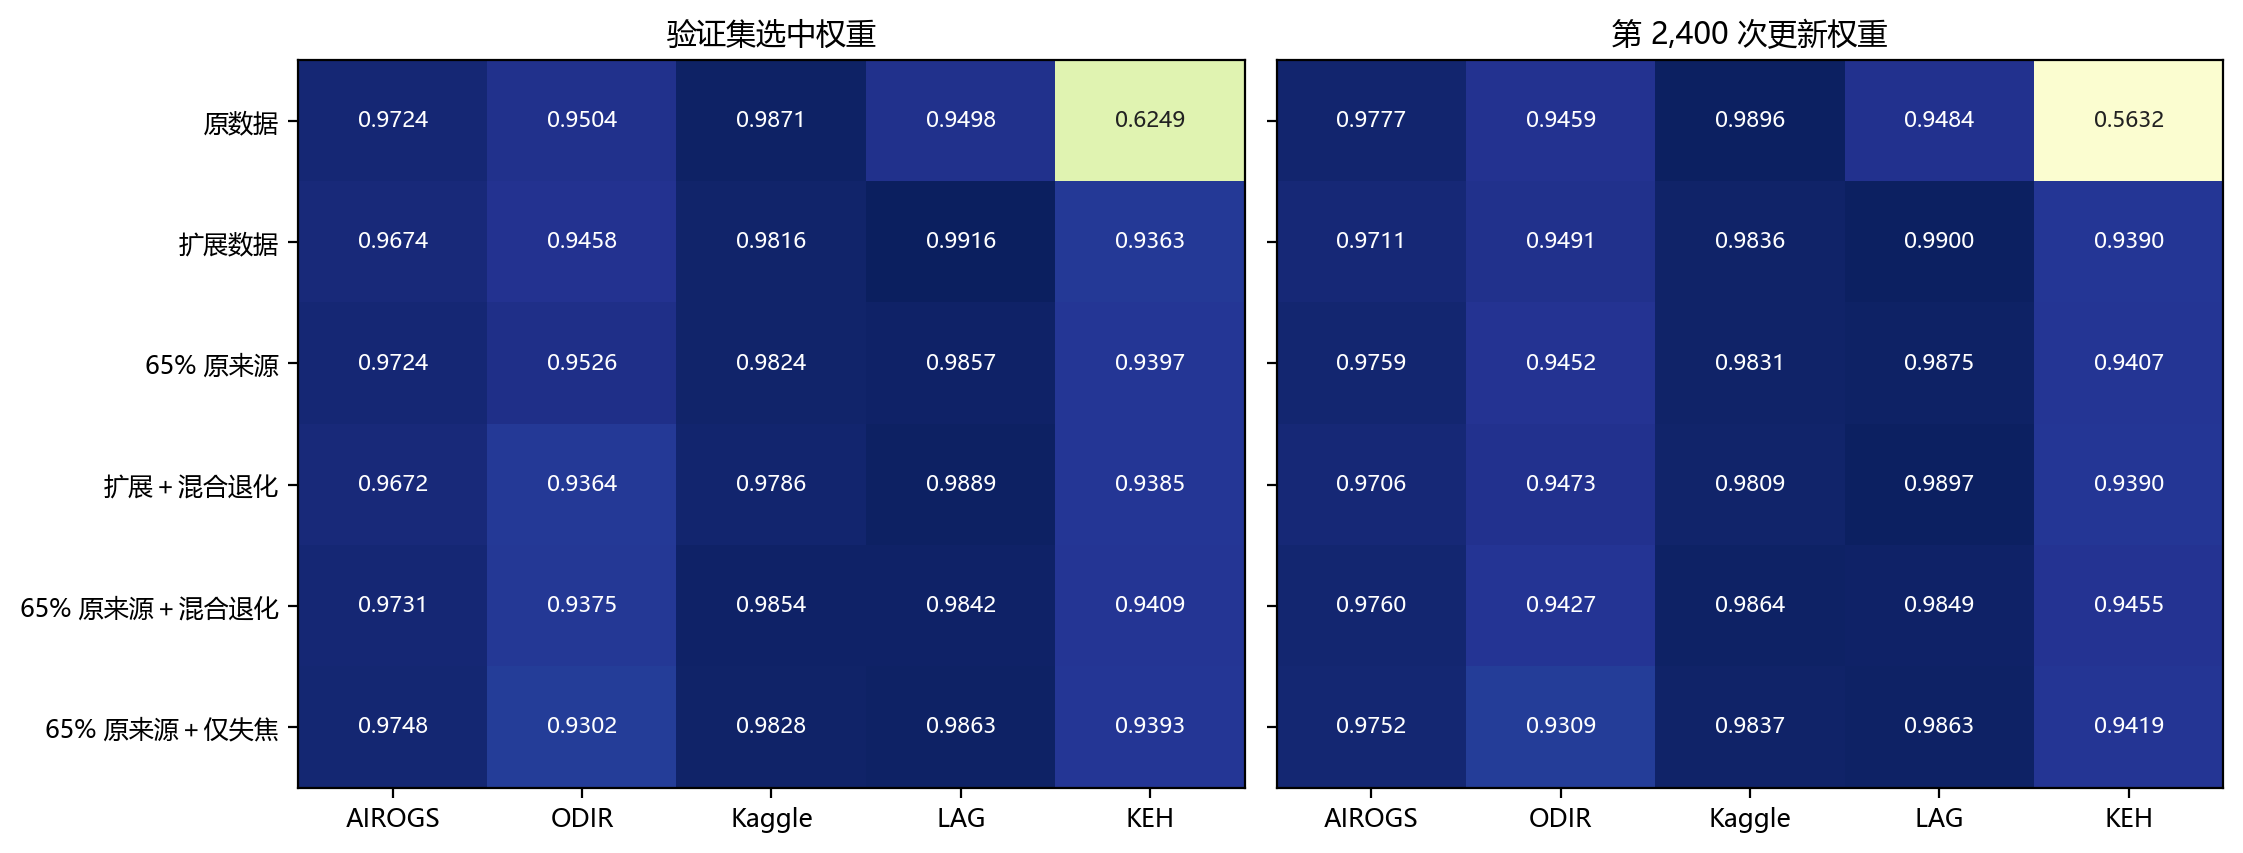
\includegraphics[keepaspectratio,alt={两个训练阶段的来源 AUROC}]{source-auroc.zh.png}}
\caption{两个训练阶段的来源 AUROC}
\end{figure}

图 1 每个格子是同一来源、三个种子的平均疾病
AUROC。左侧使用验证集选中权重，右侧统一使用第 2,400
次更新权重，颜色越深表示排序越好。两个训练阶段分别回答``按既定验证标准选模后表现如何''和``相同更新预算结束时表现如何''。

选中权重下，扩展无退化使 LAG 从 0.9498 提升至 0.9916，KEH 从 0.6249
提升至 0.9363。三个种子上的 LAG 增量为 +0.0472、+0.0383、+0.0401；KEH 为
+0.2979、+0.2769、+0.3593。LAG 和 KEH
被纳入训练来源后，来源覆盖产生了明确收益。合并全部来源的开发 AUROC 从
0.9365 提高至 0.9753。

\begin{figure}[H]
\centering
\pandocbounded{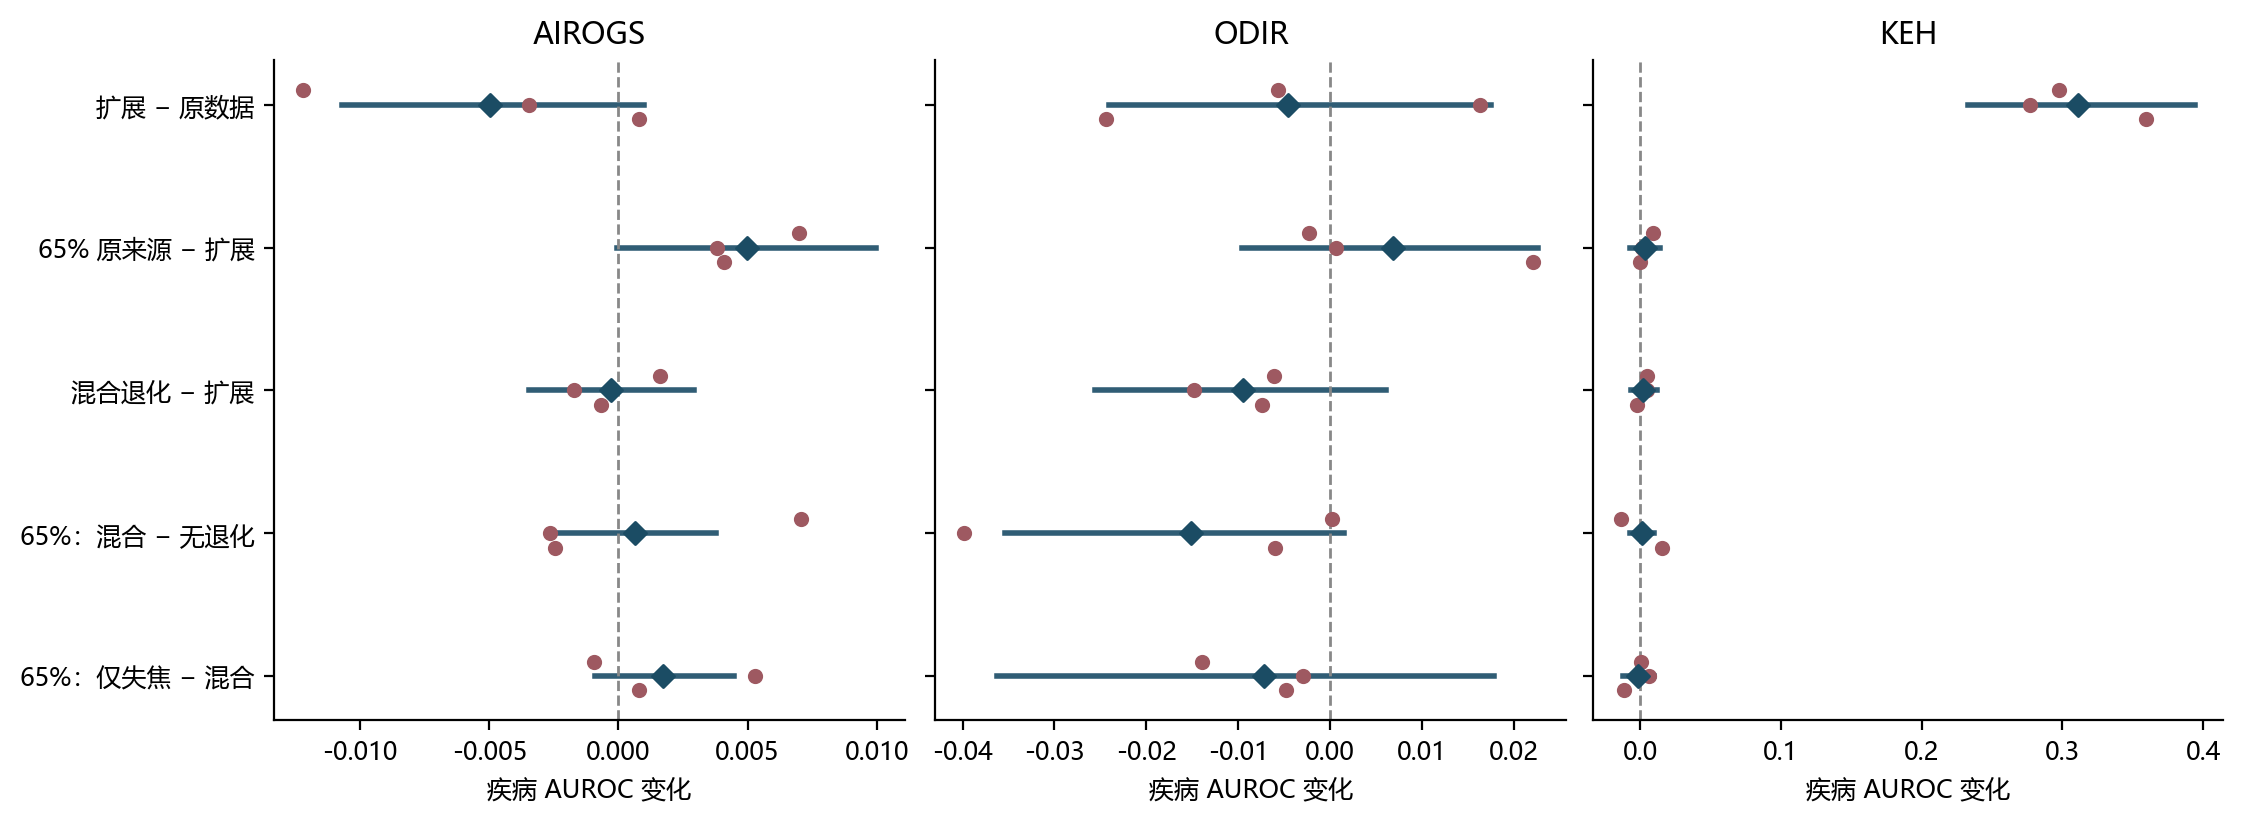
\includegraphics[keepaspectratio,alt={主要来源的配对 AUROC 变化}]{paired-source-effects.zh.png}}
\caption{主要来源的配对 AUROC 变化}
\end{figure}

图 2
红点为三个共同种子的配对变化，菱形为其均值，横线为按同一批关联组重采样
2,000 次得到的 95\%
区间。每次抽样对两方案使用相同病例，并对三个固定模型的变化取平均。横线反映病例抽样；三个点单独呈现训练种子的变化。LAG
扩展增量的病例区间为 {[}0.0280, 0.0555{]}，KEH 为 {[}0.2326, 0.3940{]}。

当前扩展采样在 2,400 次更新中，原来源平均出现 18,849 次，占 49.1\%；65\%
方案出现 24,950 次，比当前扩展采样多约
32\%。恢复这部分训练次数后，选中权重的 AIROGS AUROC
三个种子均提高，增量为 +0.0070、+0.0038、+0.0041，平均 +0.0050。同时 LAG
三个种子均下降，平均
−0.0059。这是原来源训练量与新增来源训练量之间的取舍。

ODIR 的扩展增量在三个选中模型中分别为 −0.0057、+0.0164、−0.0244；65\%
采样相对当前扩展采样分别为
−0.0023、+0.0006、+0.0222。其方向变化较大。ODIR 的阳性病例只有 28 张、19
个关联组，病例抽样区间也较宽；后续应同时报告检出率、误报和训练阶段，而不是依据某个种子的
AUROC 确定采样比例。

\subsection{为什么选中权重和训练结束结果不同}\label{ux4e3aux4ec0ux4e48ux9009ux4e2dux6743ux91cdux548cux8badux7ec3ux7ed3ux675fux7ed3ux679cux4e0dux540c}

\begin{figure}[H]
\centering
\pandocbounded{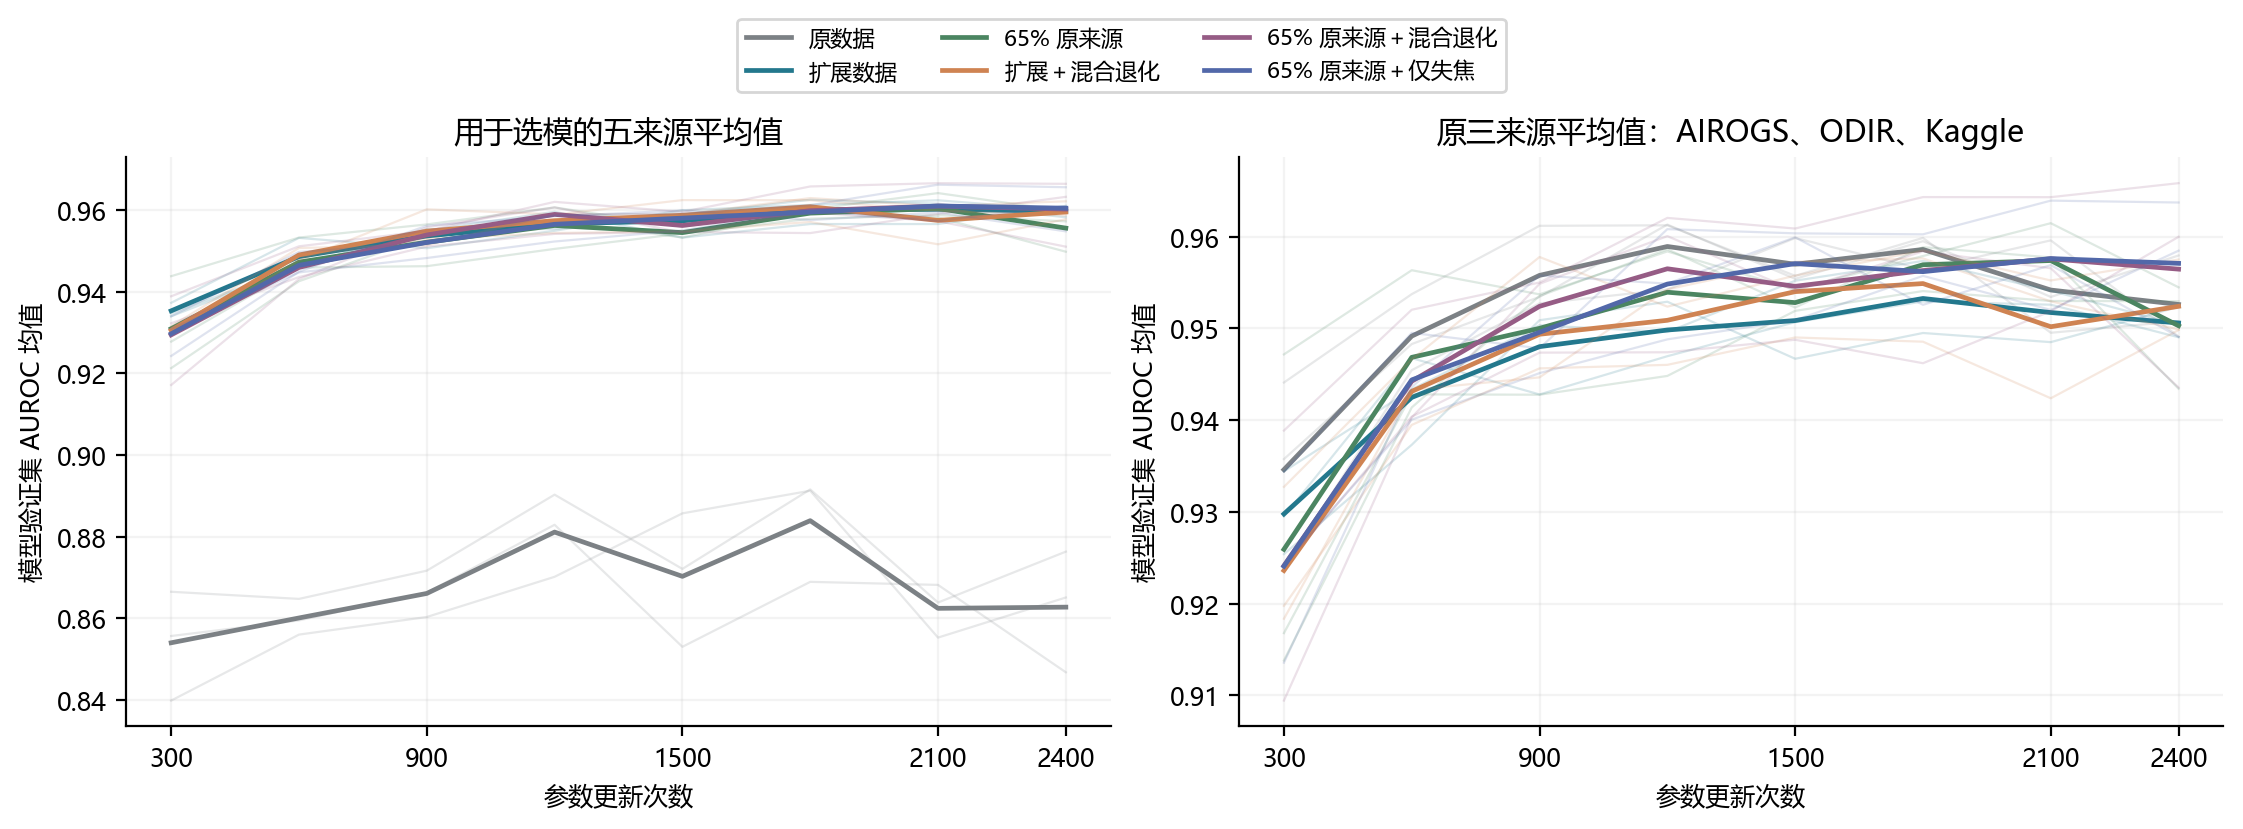
\includegraphics[keepaspectratio,alt={完整验证曲线}]{validation-curves.zh.png}}
\caption{完整验证曲线}
\end{figure}

图 3 使用 2,046
张模型验证图。粗线为三个种子的均值，细线为各个种子。左侧是用于选模的五来源
AUROC
均值，右侧只计算原三个来源。扩展方案较早提升五来源表现，后续收益逐渐变小；原数据对照的五来源均值受
KEH 影响明显。

选中更新数在 1,200--2,400 之间。以 65\%
原来源加混合退化为例，三个种子选中第 2,400、1,200、2,100
次更新；在原图开发集上的漏诊数为 78、84、68。继续到统一第 2,400
次更新后，漏诊数为 78、144、86，误报数从 76、109、101 变为
76、49、65。第二个种子的误报减少 60 张，漏诊增加 60
张，反映分数和阈值表现随训练发生变化。

相同第 2,400
次更新的来源平均值如下；各个种子和标准差保存在\href{per-seed-results.csv}{逐种子结果表}。

\Needspace{8\baselineskip}
\begin{longtable}[]{@{}lllllll@{}}
\toprule\noalign{}
方案 & AIROGS & ODIR & Kaggle & LAG & KEH & 五来源均值 \\
\midrule\noalign{}
\endhead
\bottomrule\noalign{}
\endlastfoot
原数据 & 0.9777 & 0.9459 & 0.9896 & 0.9484 & 0.5632 & 0.8850 \\
扩展数据 & 0.9711 & 0.9491 & 0.9836 & 0.9900 & 0.9390 & 0.9665 \\
65\% 原来源 & 0.9759 & 0.9452 & 0.9831 & 0.9875 & 0.9407 & 0.9665 \\
扩展＋混合 & 0.9706 & 0.9473 & 0.9809 & 0.9897 & 0.9390 & 0.9655 \\
65\%＋混合 & 0.9760 & 0.9427 & 0.9864 & 0.9849 & 0.9455 & 0.9671 \\
65\%＋失焦 & 0.9752 & 0.9309 & 0.9837 & 0.9863 & 0.9419 & 0.9636 \\
\end{longtable}

65\% 采样在这一训练阶段对 AIROGS 的平均收益为 +0.0048，对 ODIR 为
−0.0039，与选中权重的 ODIR 平均 +0.0068
方向不同。后续比较将验证集选中权重作为主结果，第 2,400
次更新作为相同训练预算的补充结果。

\subsection{退化增强：失焦收益与实际增强次数}\label{ux9000ux5316ux589eux5f3aux5931ux7126ux6536ux76caux4e0eux5b9eux9645ux589eux5f3aux6b21ux6570}

\begin{figure}[H]
\centering
\pandocbounded{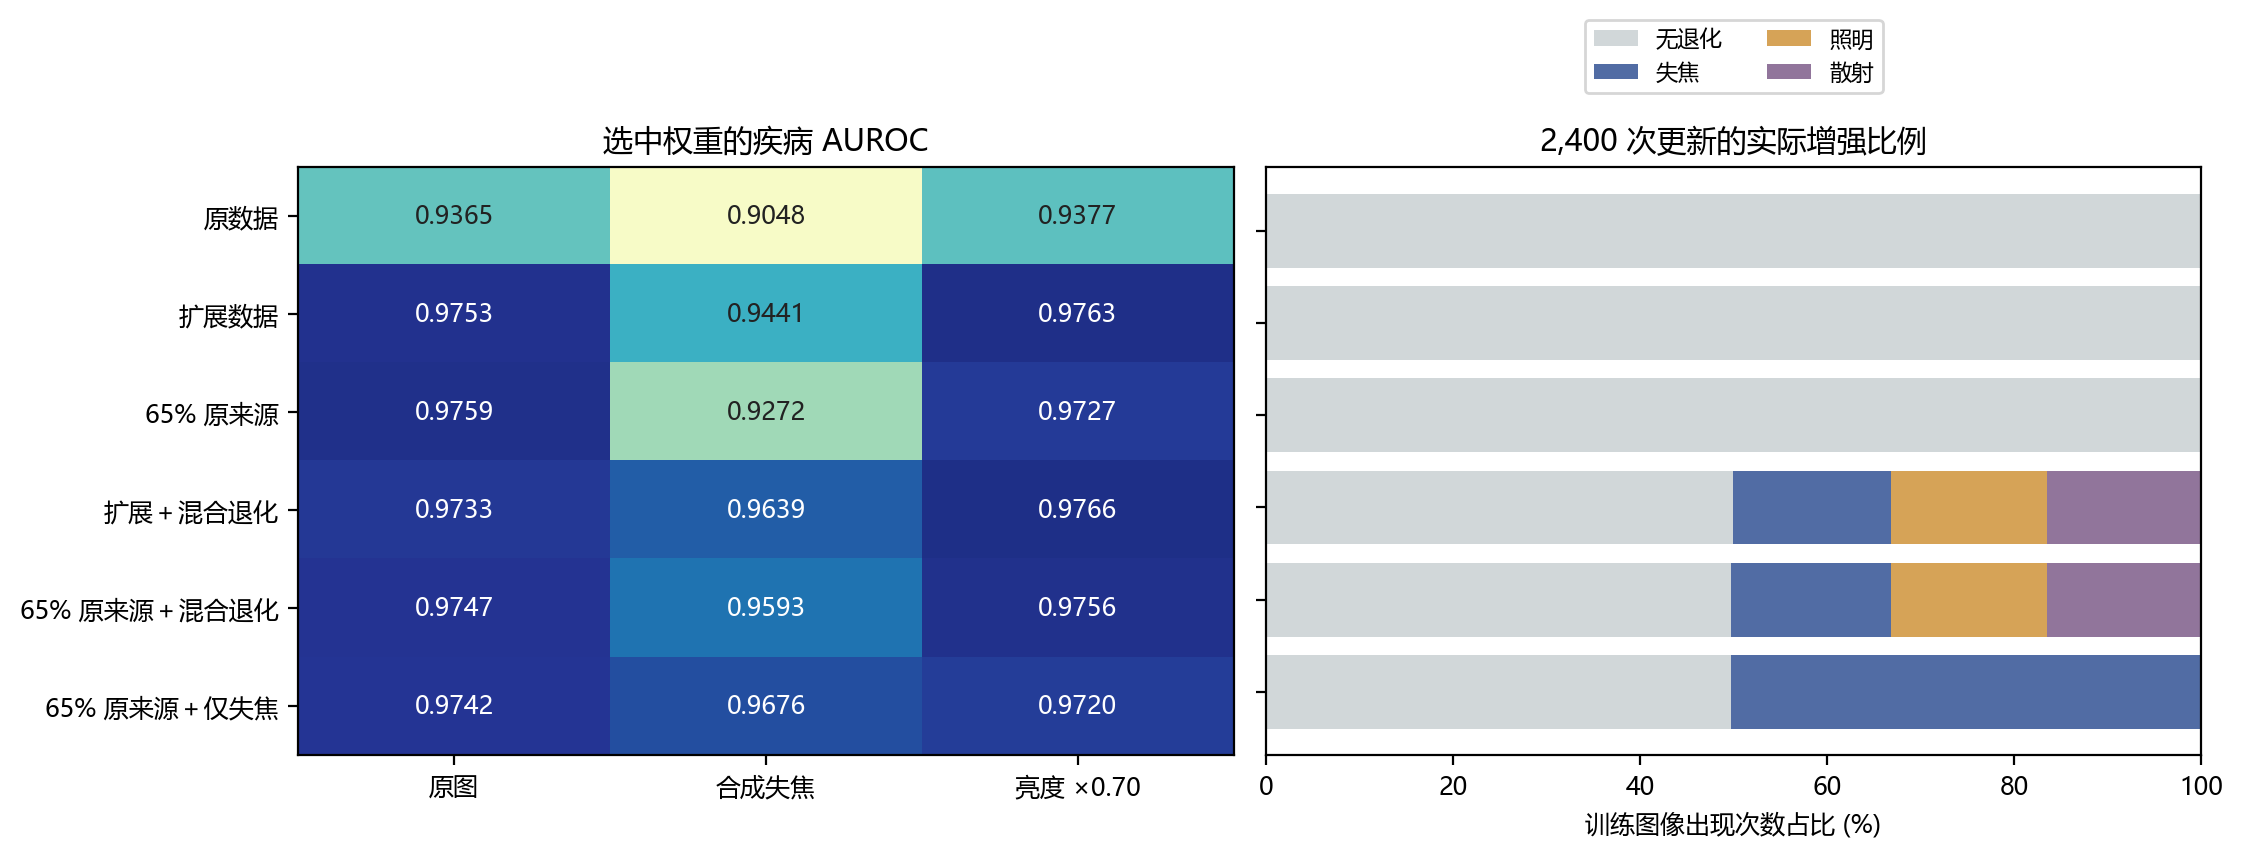
\includegraphics[keepaspectratio,alt={合成压力集表现与增强次数}]{stress-and-training-dose.zh.png}}
\caption{合成压力集表现与增强次数}
\end{figure}

图 4 左侧使用选中权重：原图有 2,053 张，两个合成条件各使用相同 384
张原图，包括 146 张阳性、238
张阴性。失焦为按可见视野直径缩放的高斯模糊，亮度条件将原图亮度乘以
0.70。右侧按全部 2,400 次更新记录的图像出现次数展示增强组成。

当前扩展采样下，混合退化相对无退化的失焦 AUROC
在三个种子均提高，平均增加 0.0197，病例抽样区间为 {[}0.0086,
0.0316{]}；65\% 采样下平均增加 0.0321。65\% 原来源仅失焦的失焦 AUROC 为
0.9676，高于对应混合方案的 0.9593，三个种子均提高。原图五来源均值则从
0.9642 降至 0.9627，亮度条件从 0.9756 降至 0.9720。

增强频率解释了这组比较的一部分。混合方案中失焦约占全部训练图像出现次数的
17\%，仅失焦方案约占 50\%；首个种子分别为 6,554 次和 19,341 次，相差
2.95
倍。因此，目前比较同时改变增强组成和失焦出现次数。进一步分解机制时，应增加约六分之一概率的仅失焦方案，与混合方案匹配失焦次数。

失焦还会推动阳性、阴性分数向彼此靠近。在扩展无退化模型中，同一原图合成失焦后，阴性
p 平均上移 0.0590，阳性下移 0.0761；混合退化后两者为 +0.0280 和
−0.0617。增强减轻了这一分数变化，尤其减少阴性分数上移。真实低质量病例的检出将在人工质量分层中单独评价。

\subsection{漏诊、误报与分类阈值}\label{ux6f0fux8bcaux8befux62a5ux4e0eux5206ux7c7bux9608ux503c}

\begin{figure}[H]
\centering
\pandocbounded{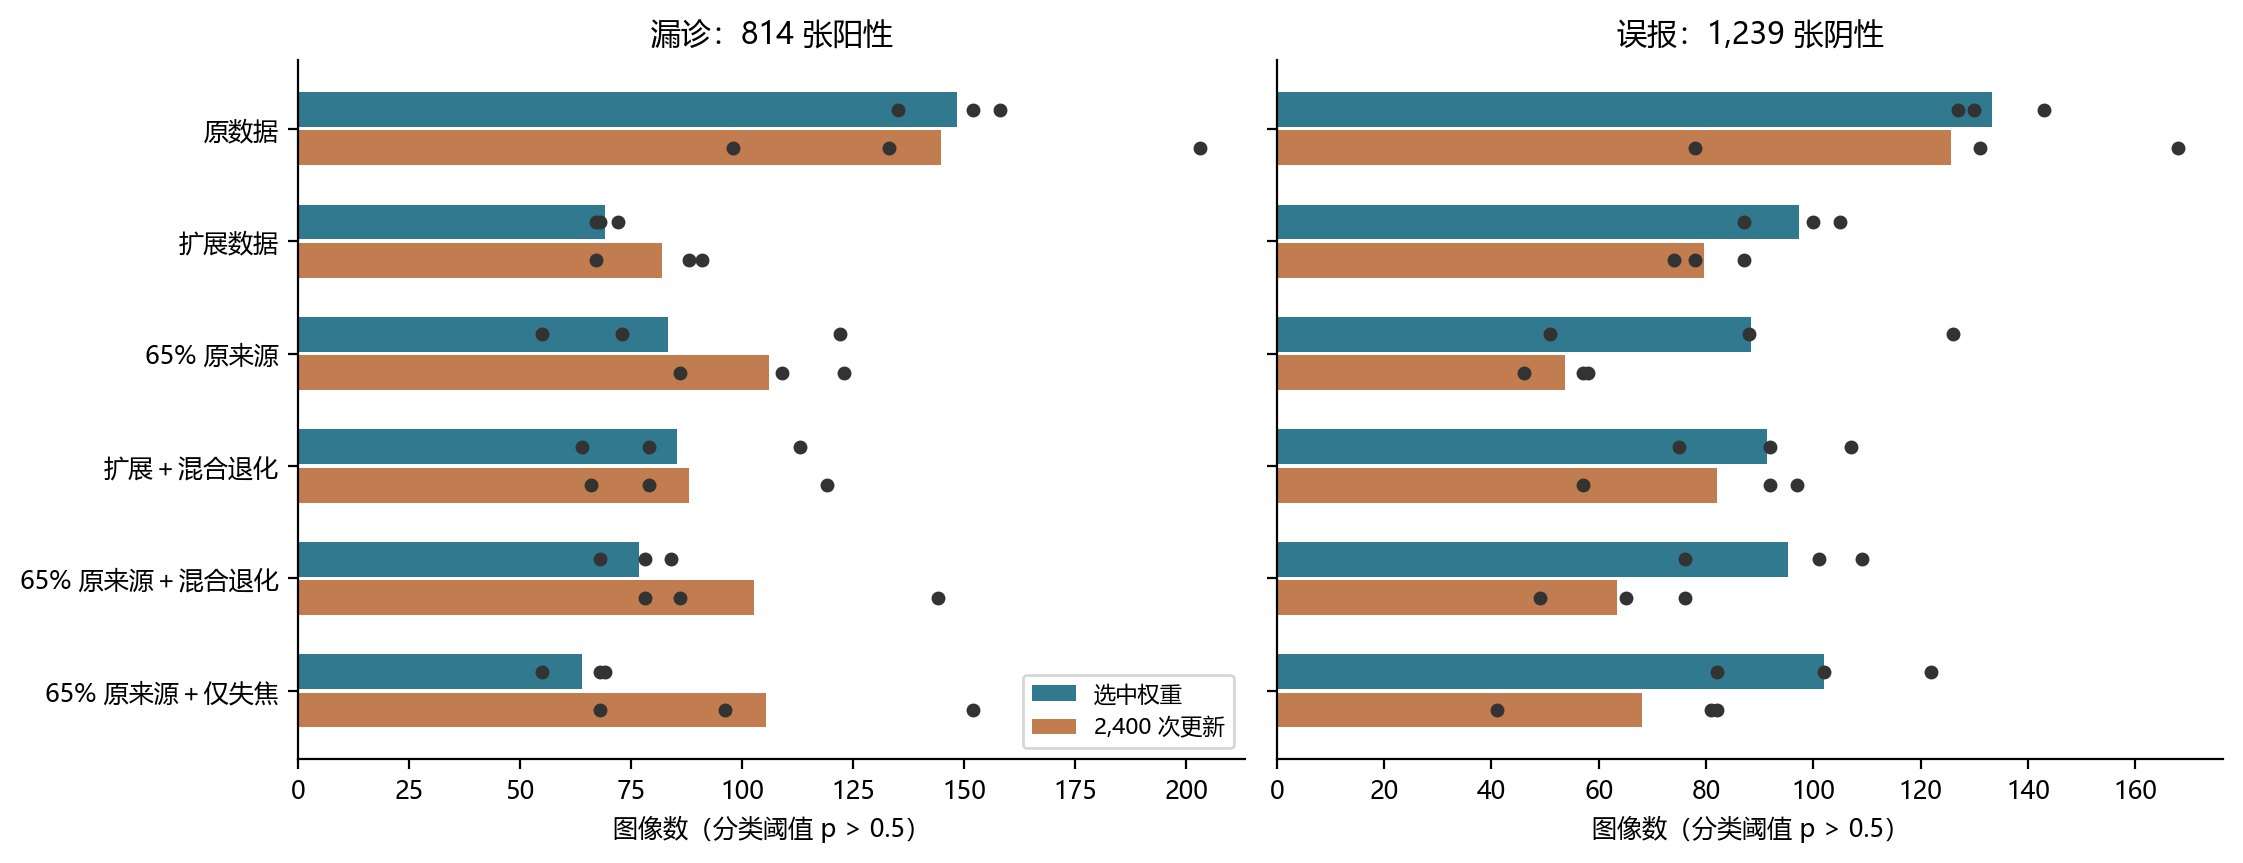
\includegraphics[keepaspectratio,alt={原图漏诊和误报}]{misses-and-false-alarms.zh.png}}
\caption{原图漏诊和误报}
\end{figure}

图 5 使用相同 2,053 张规则开发原图、分类阈值
0.5。柱为三个种子的平均计数，黑点为各个种子；蓝色是选中权重，棕色是第
2,400 次更新。漏诊以 814 张阳性为分母，误报以 1,239 张阴性为分母。

选中权重下，扩展无退化平均漏诊 69.0 张、误报 97.3 张；65\%
原来源加混合退化为 76.7 和 95.3；仅失焦为 64.0 和
102.0。按当前阈值，仅失焦偏向多检出阳性，代价是更多误报。第 2,400
次更新下，65\% 无退化方案相比扩展无退化少 26.0 个误报、多 24.0
个漏诊，总错误数差为 -2.0。总错误数需要与这两类错误分别阅读。

另以每个来源的验证阴性分数第 95
百分位确定阈值，再固定用于规则开发原图，得到下表。表中为三个种子的平均结果；规则开发集的实际特异度由表中数据给出。

\Needspace{8\baselineskip}
\begin{longtable}[]{@{}lll@{}}
\toprule\noalign{}
方案 / 来源 & 检出率 & 特异度 \\
\midrule\noalign{}
\endhead
\bottomrule\noalign{}
\endlastfoot
扩展数据 / AIROGS & 83.7\% & 94.3\% \\
扩展数据 / ODIR & 57.1\% & 96.4\% \\
65\%＋混合 / AIROGS & 84.6\% & 94.5\% \\
65\%＋混合 / ODIR & 48.8\% & 97.1\% \\
65\%＋失焦 / AIROGS & 87.3\% & 94.1\% \\
65\%＋失焦 / ODIR & 46.4\% & 96.4\% \\
\end{longtable}

ODIR 在这一阈值比较下，扩展无退化检出率为 57.1\%，65\% 加混合退化为
48.8\%，仅失焦为 46.4\%。分类 AUROC
较高仍会与某个阈值下的低检出率同时出现。接下来的阈值选择应明确可接受的漏诊率，并展示对应的误报和复核工作量。

\subsection{质量与错误的关系在完整实验中如何变化}\label{ux8d28ux91cfux4e0eux9519ux8befux7684ux5173ux7cfbux5728ux5b8cux6574ux5b9eux9a8cux4e2dux5982ux4f55ux53d8ux5316}

\begin{figure}[H]
\centering
\pandocbounded{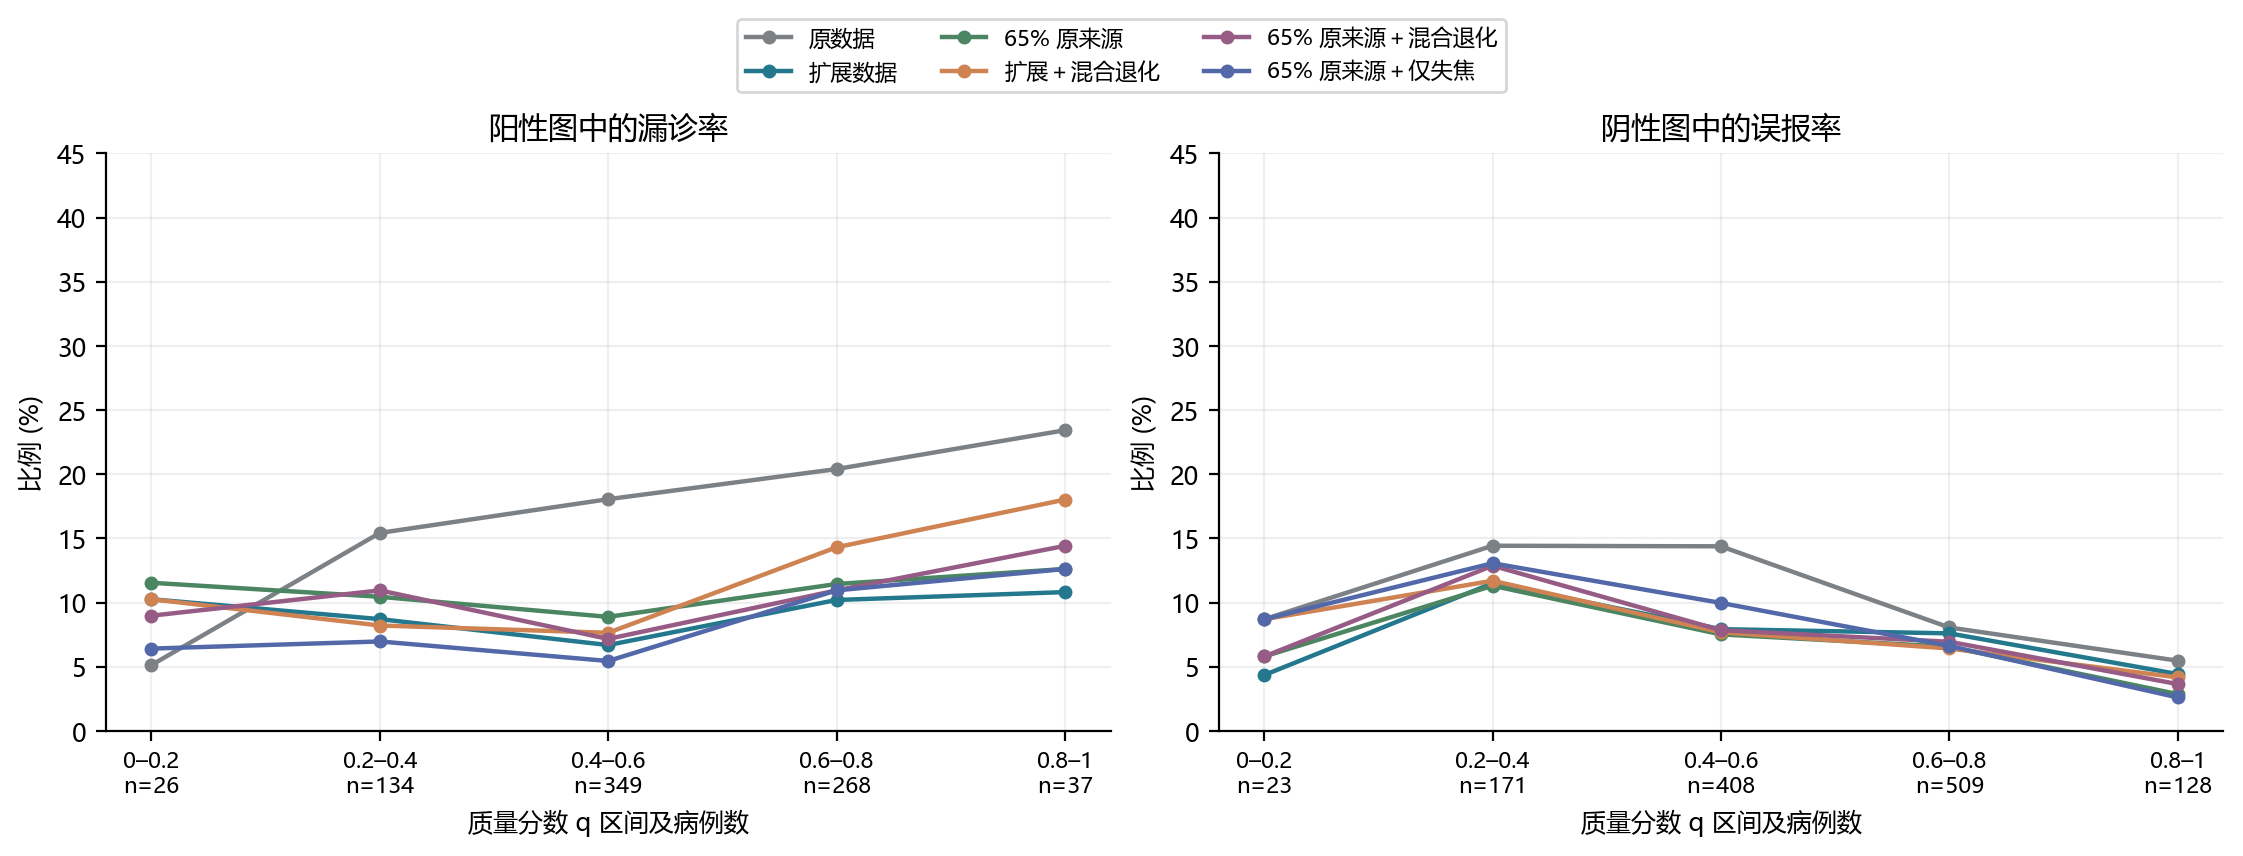
\includegraphics[keepaspectratio,alt={按质量区间分别计算漏诊率和误报率}]{quality-error-rates.zh.png}}
\caption{按质量区间分别计算漏诊率和误报率}
\end{figure}

图 6 使用原 FTHNet 质量分数 q 和 18
个选中疾病模型。线为每个方案三个种子的平均错误率，横轴下方 n
是每个区间的阳性或阴性图像数，同一批病例在各种子中重复评价。漏诊率和误报率分别按疾病类别计算。

低 q 区间的阳性、阴性组成不同。q \textless{} 0.2 只有 26 张阳性和 23
张阴性，而 q ≥ 0.4 有 654 张阳性、1,045 张阴性。中高 q
区域的大量错误首先与病例数量相对应。按阳性计算的漏诊率在最高 q
区间仍较高：65\% 加混合退化三个种子分别漏诊
6/37、6/37、4/37。全图质量较好也可能伴随疾病判断困难。

\begin{figure}[H]
\centering
\pandocbounded{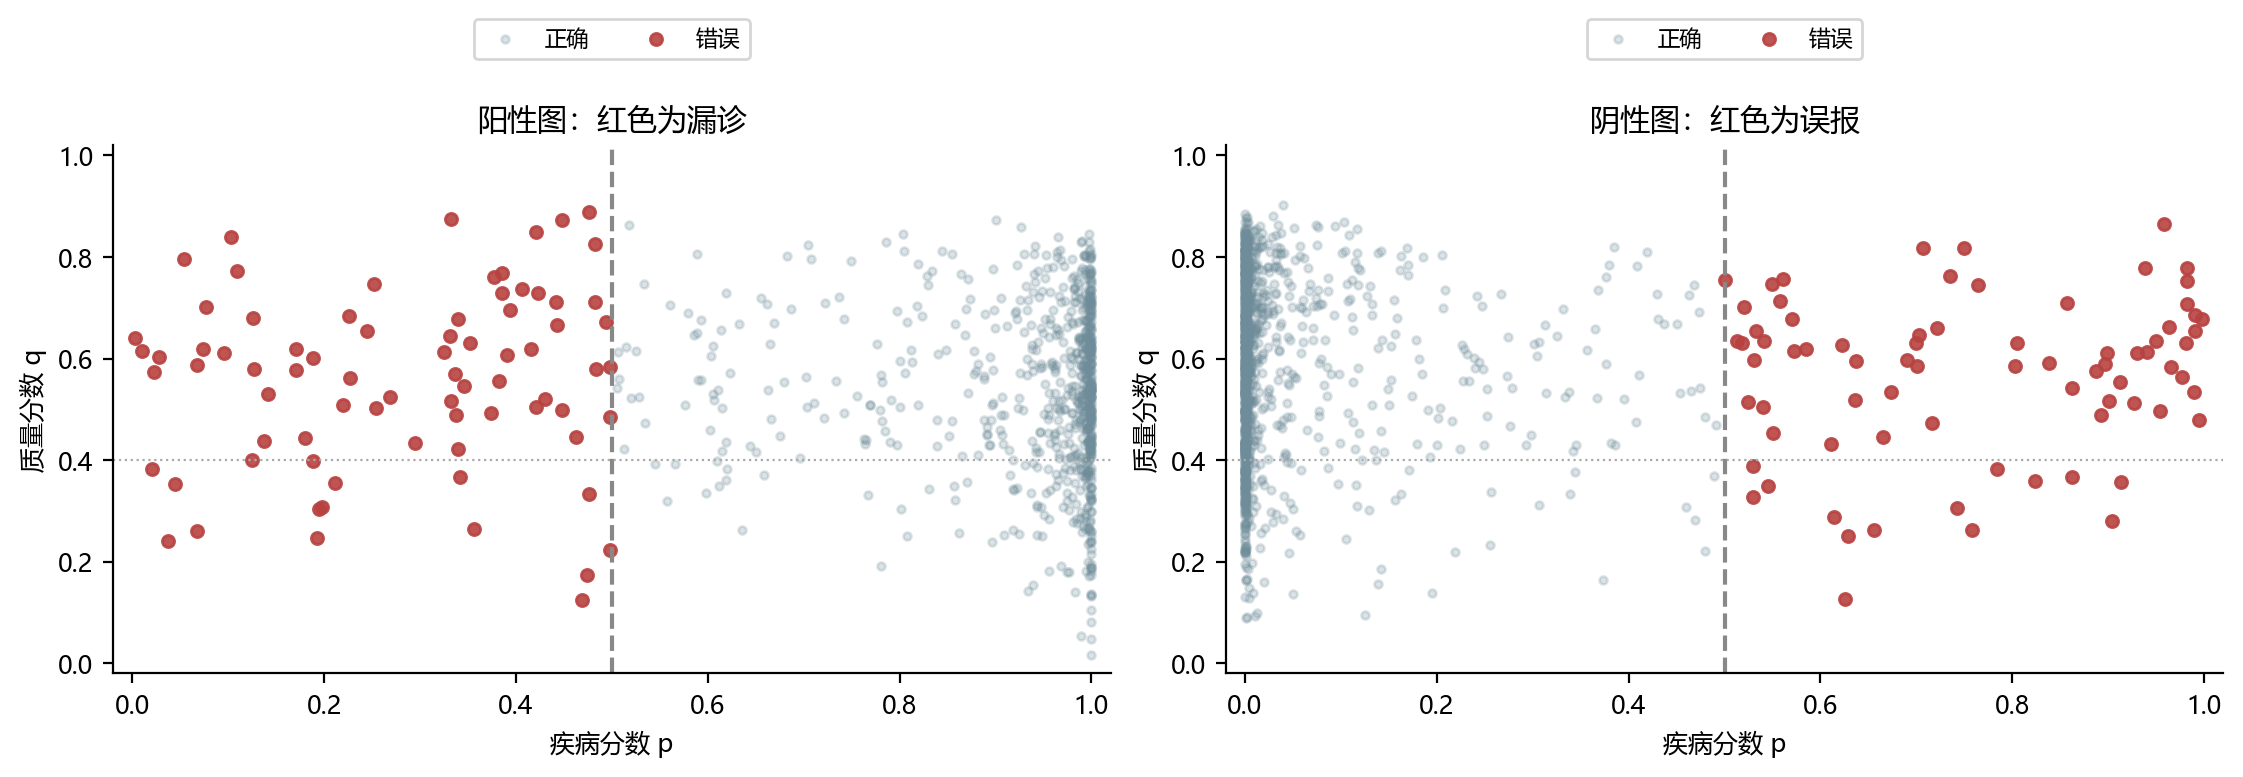
\includegraphics[keepaspectratio,alt={疾病分数与质量分数的联合分布}]{disease-quality-distribution.zh.png}}
\caption{疾病分数与质量分数的联合分布}
\end{figure}

图 7 展示按验证标准表现最高的方案------65\%
原来源加混合退化------首个种子第 2,400
次更新的规则开发结果。蓝灰点为正确分类，红点为错误；左侧仅阳性，右侧仅阴性。竖线
p=0.5 是本次分类阈值，横线 q=0.4
用于比较质量分数范围。漏诊和误报分布在不同质量水平，复核区域需要结合
p、q 及两类错误分别评价。

\subsection{加入质量分数的复核收益}\label{ux52a0ux5165ux8d28ux91cfux5206ux6570ux7684ux590dux6838ux6536ux76ca}

每个固定疾病模型使用五折分组交叉验证拟合错误排序：同一关联组的图像进入同一折，用其余四折拟合，再为留出折生成预测。逻辑回归学习输入分数与出错概率之间的关系；仅
p 的方法使用疾病分数的正负方向和距 0.5 的程度，加入 q
后进一步学习质量与疾病分数的共同作用。两种方法在同一模型上使用相同分折，标准化在训练折内计算。另用第
17 轮选中的 EyeQ 质量模型重复比较。

下表的 AUROC
衡量识别错误的排序能力：随机抽取一张错误图和一张正确图，分数将错误排在前面的概率，0.5
为随机水平。前三个指标为各方案三个种子的平均值；最后一列依次给出三个种子在复核
411 张图时，加入 FTHNet q 相对仅 p 拟合多选中的错误数。

\Needspace{8\baselineskip}
\begin{longtable}[]{@{}
  >{\raggedright\arraybackslash}p{(\linewidth - 8\tabcolsep) * \real{0.2000}}
  >{\raggedright\arraybackslash}p{(\linewidth - 8\tabcolsep) * \real{0.2000}}
  >{\raggedright\arraybackslash}p{(\linewidth - 8\tabcolsep) * \real{0.2000}}
  >{\raggedright\arraybackslash}p{(\linewidth - 8\tabcolsep) * \real{0.2000}}
  >{\raggedright\arraybackslash}p{(\linewidth - 8\tabcolsep) * \real{0.2000}}@{}}
\toprule\noalign{}
\begin{minipage}[b]{\linewidth}\raggedright
方案
\end{minipage} & \begin{minipage}[b]{\linewidth}\raggedright
仅低 q AUROC
\end{minipage} & \begin{minipage}[b]{\linewidth}\raggedright
p 不确定性 AUROC
\end{minipage} & \begin{minipage}[b]{\linewidth}\raggedright
加入 q：AUROC 差
\end{minipage} & \begin{minipage}[b]{\linewidth}\raggedright
加入 q：多选中错误
\end{minipage} \\
\midrule\noalign{}
\endhead
\bottomrule\noalign{}
\endlastfoot
原数据 & 0.5433 & 0.8277 & -0.0007 & -4 / -1 / +0 \\
扩展数据 & 0.5235 & 0.8822 & -0.0003 & +0 / +1 / +4 \\
65\% 原来源 & 0.5402 & 0.8859 & -0.0008 & -2 / -3 / +2 \\
扩展＋混合 & 0.5110 & 0.8821 & -0.0005 & +2 / -1 / +0 \\
65\%＋混合 & 0.5364 & 0.8879 & -0.0008 & +2 / +1 / +0 \\
65\%＋失焦 & 0.5392 & 0.8749 & +0.0002 & -1 / -3 / +1 \\
\end{longtable}

\begin{figure}[H]
\centering
\pandocbounded{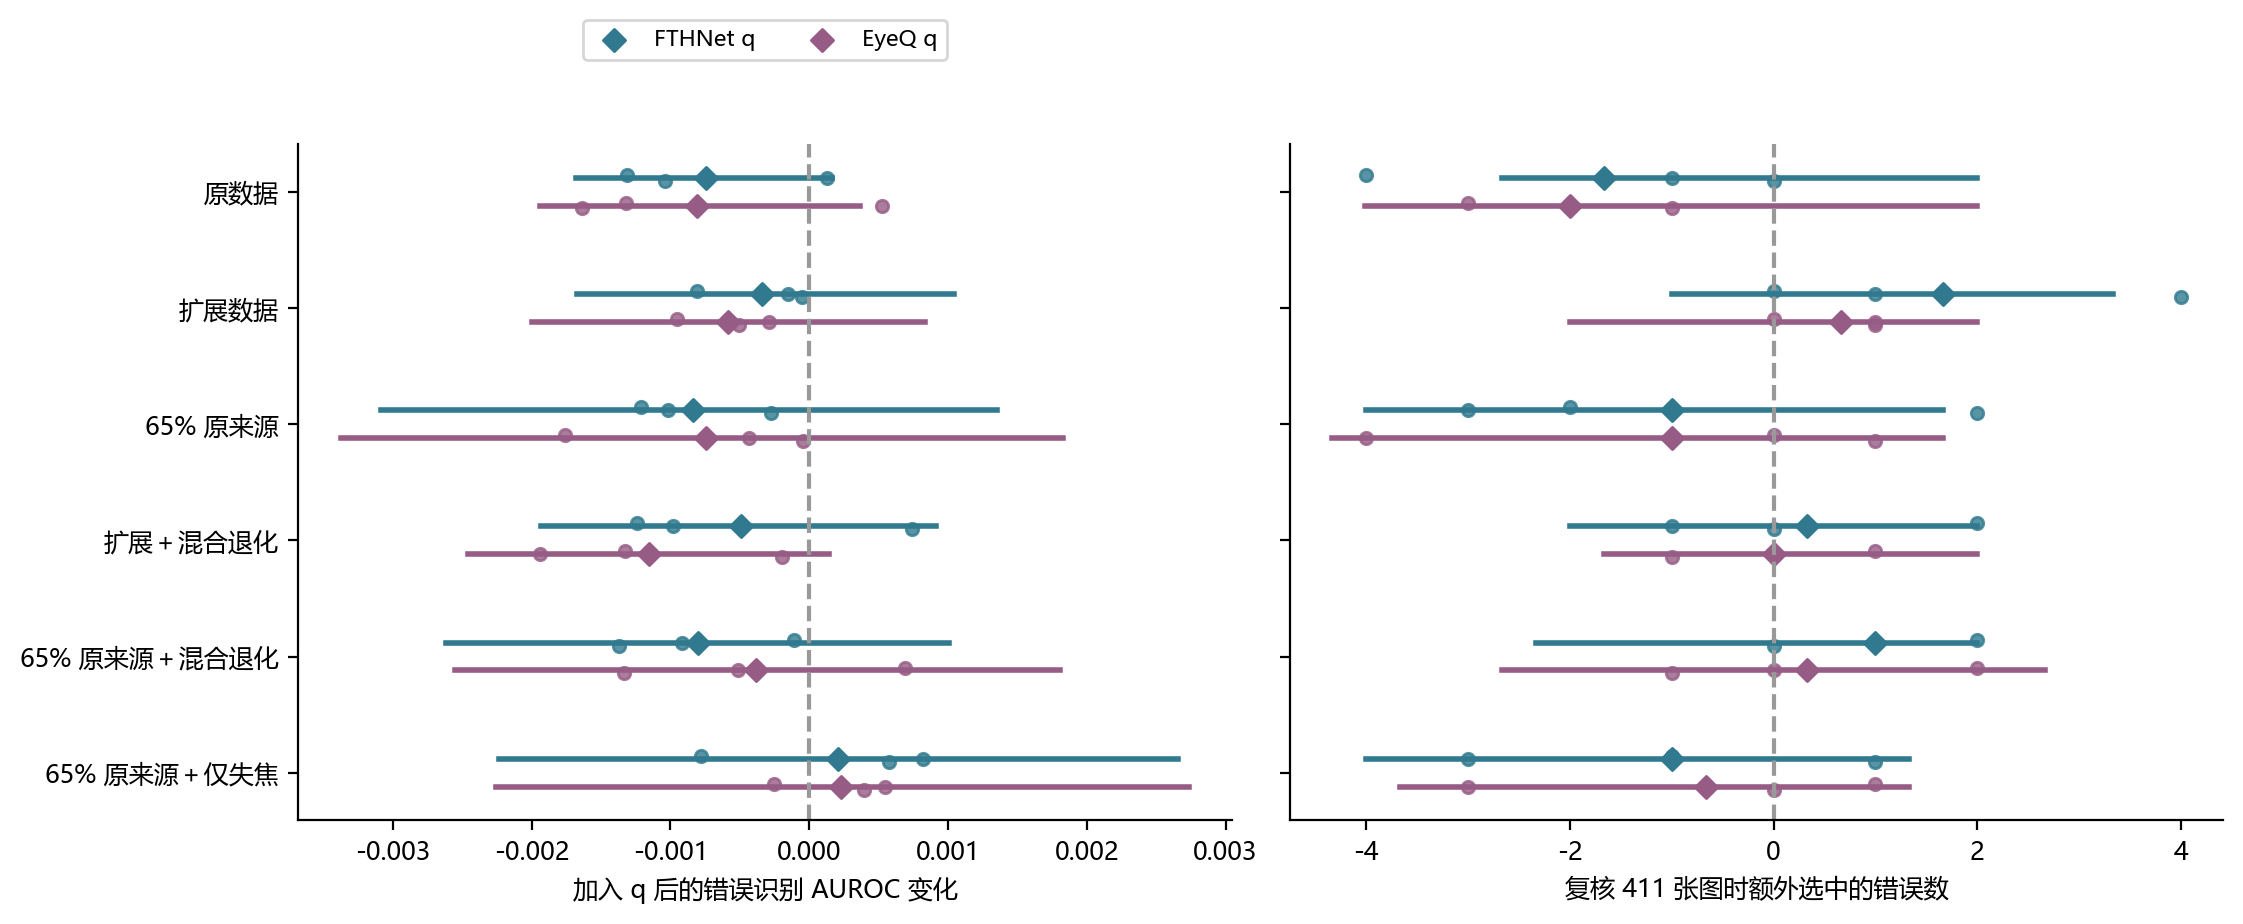
\includegraphics[keepaspectratio,alt={两套质量分数的额外复核效果}]{quality-review-effects.zh.png}}
\caption{两套质量分数的额外复核效果}
\end{figure}

图 8 各方案有 FTHNet 和 EyeQ 两组结果。点为三个种子，菱形为均值，横线为
2,000 次关联组配对抽样的 95\%
区间；每次抽样都重新排序，两方法复核张数保持相同。区间固定疾病模型和交叉验证生成的错误风险分数，评价病例抽样变化。

65\% 加混合退化中，加入 FTHNet q 的平均错误 AUROC 差为
-0.00080，病例区间为 {[}-0.00262, +0.00101{]}；20\% 复核时多选中 2、1、0
个错误，平均 +1，病例区间为 {[}−2.33, +2.00{]}。换用 EyeQ
后增量也较小。为错误模型加入来源指标后，q 的增量方向仍在不同种子间变化。

\begin{figure}[H]
\centering
\pandocbounded{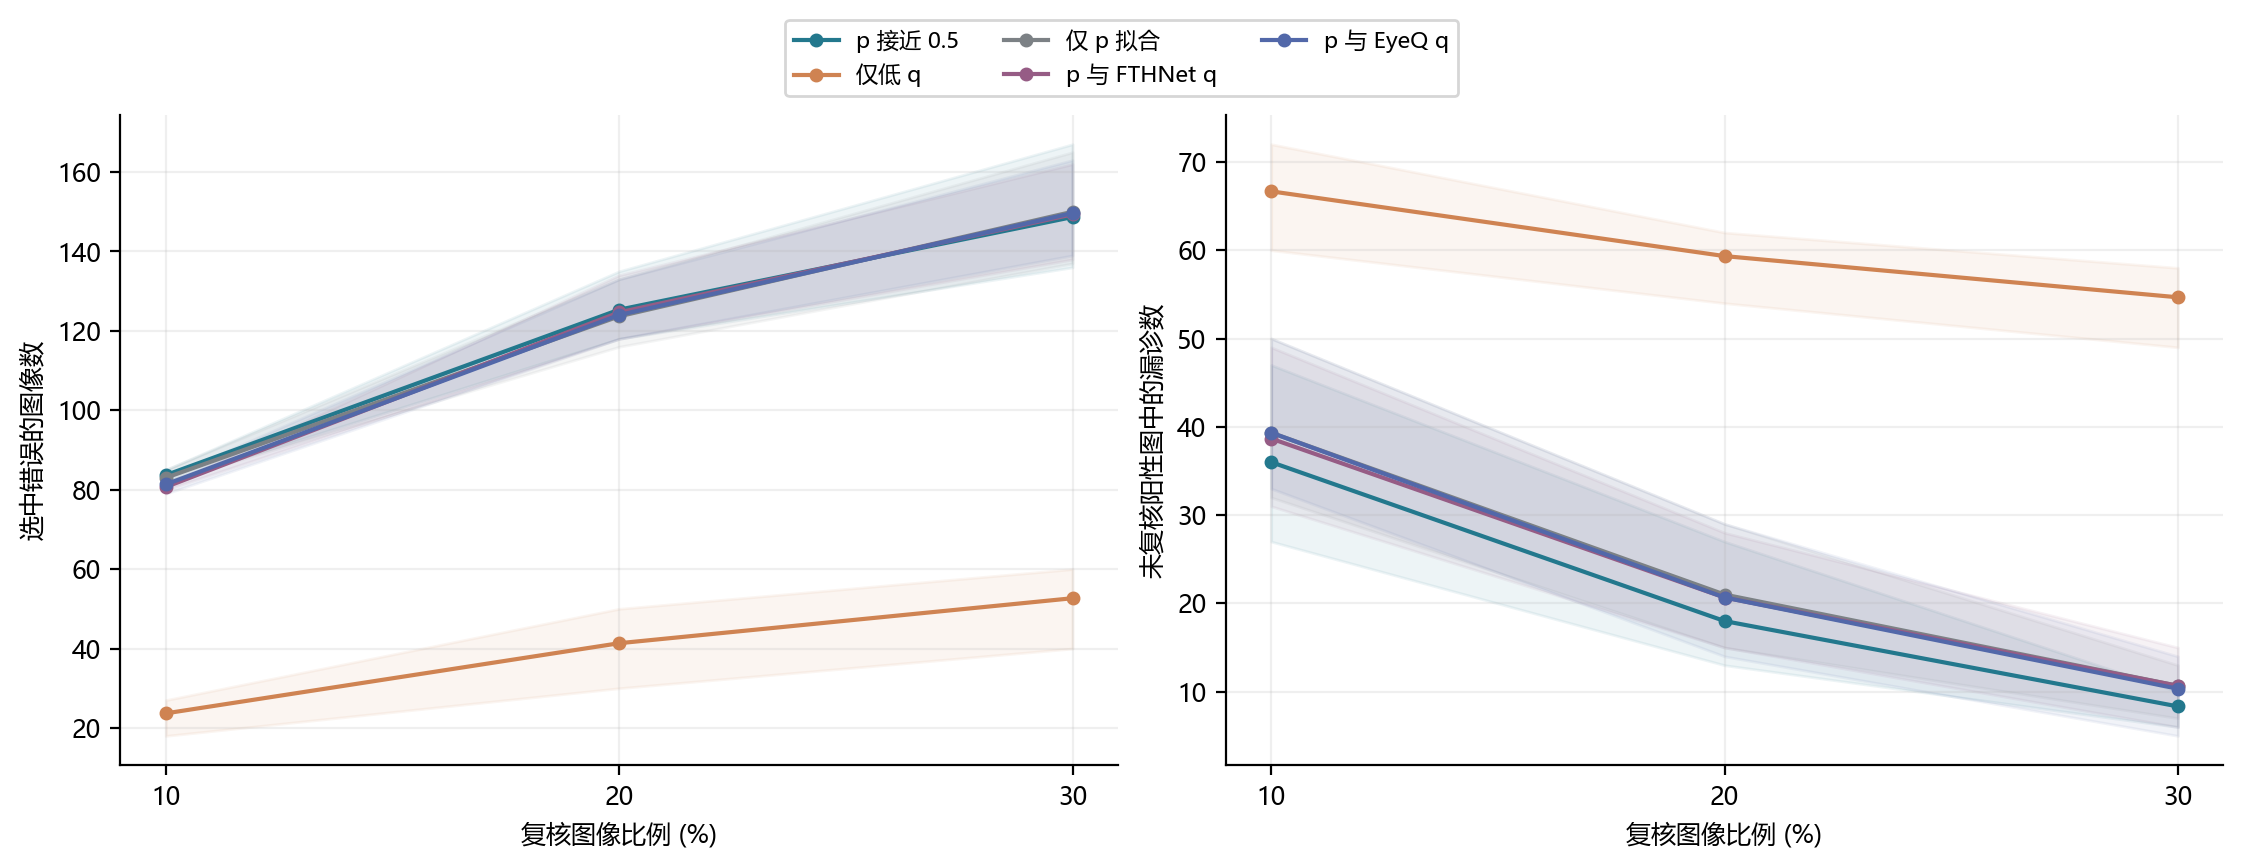
\includegraphics[keepaspectratio,alt={复核工作量与选中错误、剩余漏诊}]{review-workload.zh.png}}
\caption{复核工作量与选中错误、剩余漏诊}
\end{figure}

图 9 使用 65\%
加混合退化的三个选中模型。线为平均值，浅色范围为三种子的最小值至最大值。左侧表示送去复核的错误，右侧表示未送复核的阳性漏诊，均按照片计数。

在相同 411
张复核量下，各方法结果如下。整数计数在三个模型间取平均，因此表中可能出现小数。

\Needspace{8\baselineskip}
\begin{longtable}[]{@{}llll@{}}
\toprule\noalign{}
复核方式 & 选中错误 & 选中漏诊 & 未复核漏诊 \\
\midrule\noalign{}
\endhead
\bottomrule\noalign{}
\endlastfoot
p 接近 0.5 & 125.3 & 58.7 & 18.0 \\
仅低 q & 41.3 & 17.3 & 59.3 \\
仅 p 拟合 & 123.7 & 55.7 & 21.0 \\
p 与 FTHNet q & 124.7 & 56.0 & 20.7 \\
p 与 EyeQ q & 124.0 & 56.0 & 20.7 \\
\end{longtable}

p 接近 0.5 的简单排序平均选中 125.3 个错误、58.7 个漏诊，未复核漏诊为
18.0；拟合 p、q 后分别为
124.7、56.0、20.7。照片质量识别与疾病错误识别是两项不同任务；本轮复核收益以疾病分数提供的信息为主。后续项目提案中的比较保留简单
p 排序和同一模型的仅 p 拟合作为对照，以额外捕获错误、漏诊和复核量判断 q
的价值。

\subsection{真实低质量样本如何影响结果}\label{ux771fux5b9eux4f4eux8d28ux91cfux6837ux672cux5982ux4f55ux5f71ux54cdux7ed3ux679c}

\begin{figure}[H]
\centering
\pandocbounded{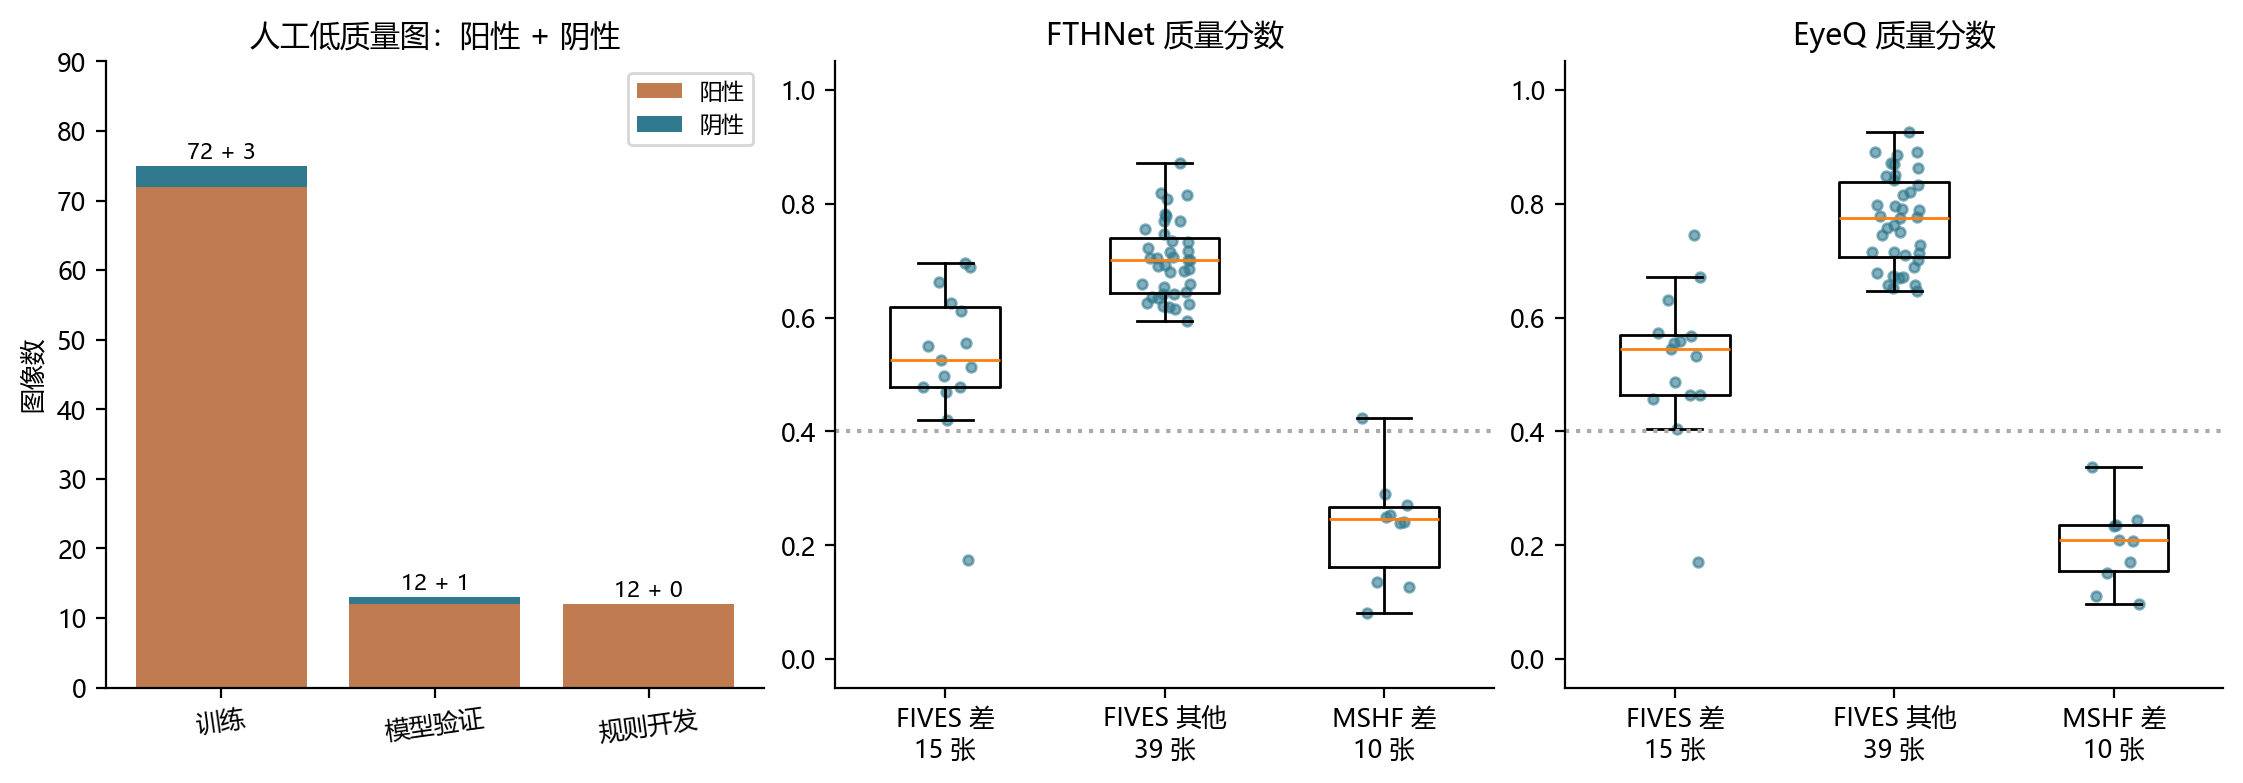
\includegraphics[keepaspectratio,alt={人工质量病例组成与两套质量模型分数}]{real-quality-composition.zh.png}}
\caption{人工质量病例组成与两套质量模型分数}
\end{figure}

图 10 左侧汇总 FIVES、MSHF 人工低质量图的用途和疾病类别，柱顶为阳性 +
阴性。右侧使用模型验证和规则开发合计的 FIVES 54 张、MSHF 10
张原图；点为照片，箱体为四分位范围，中线为中位数。FIVES
的差质量定义是至少一个质量维度为差，MSHF 使用官方总体质量。

训练中有 72 张人工低质量阳性、3 张阴性；规则开发中有 12 张阳性、0
张阴性，模型验证仅 1 张低质量阴性。全部 15 个扩展模型均检出这 12
张阳性，原数据对照分别漏诊 5、5、4 张。无退化扩展也达到
12/12，表明这组病例的检出提升已经随数据扩展出现。12
个病例零漏诊对应的单侧 95\% 漏诊率上界为
22.1\%；低质量误报则需要独立阴性病例来估计。

样本不足包含两部分：低质量病例总数少，以及低质量与疾病标签、来源强相关。重复采样增加的是同一病例的训练次数，合成退化增加的是既有病例的变换；真实低质量阴性补样能同时改善训练组成和误报评价。补样优先寻找同来源、同采集条件、有明确青光眼阴性诊断及人工质量等级的独立病例。若无错误，分别至少
59 个独立阳性和 59 个独立阴性可使单侧 95\% 错误率上界低于
5\%；它们是后续收集规划的最低参照。

质量等级与连续分数还需按来源解释。FIVES 的 15 张人工低质量开发图 q
中位数为 0.5261，只有 1 张 q\textless0.4；MSHF 的 10 张低质量图中位数为
0.2453，9 张 q\textless0.4。FTHNet 在 FIVES 内辨认人工低质量的 AUROC 为
0.9026，EyeQ 为
0.9641。两套模型具有质量区分能力，当前较弱的是质量分数对疾病错误的额外排序信息。下一步人工复核应同时记录全图质量和视盘诊断信息是否可见。

\subsection{后续安排}\label{ux540eux7eedux5b89ux6392}

按预先使用的五来源验证均值，65\%
原来源加混合退化为后续候选方案，三种子均值为
0.9634；该方案内验证值最高的是种子 20261117、第 2,100 次更新，验证均值
0.9665。扩展无退化保留为数据扩展和质量复核的主要对照。该方案的三种子平均全体开发
AUROC 为 0.9747，分类阈值 0.5 时平均漏诊 76.7、误报 95.3。

优先推进三项工作：一是补充真实低质量阴性及独立阳性，分来源建立质量评价层；二是选择分类阈值并比较相同复核量下的残余漏诊和误报，维持疾病分数对照；三是匹配失焦出现次数，分解混合增强中的失焦频率与其他处理的作用。模型、阈值和复核区域确定后，按冻结用途进行最终测试。

本轮数据与图表见\href{completed-analysis.json}{分析
JSON}、\href{per-seed-results.csv}{逐种子
CSV}；方法见\href{../../../../tools/analyze_completed_followup_20261115.py}{分析程序}和\href{../../../../tools/report_completed_followup_20261115.py}{报告程序}。\href{../../../../runs/followup_20261115/pipeline/status.json}{执行状态}记录
18
组完成，\href{../quality-and-training.zh.md}{早期质量分析}保留训练启动时的快照。中英文
Markdown、PDF、LaTeX 和十组双语图表保存在本目录。

\end{document}
